\section{Analisi degli investimenti}
\subsection{Modello WACC}
Per determinare il tasso di sconto si è deciso di utilizzare il modello
"WACC - Weighted Average Cost of Capital", per poter tenere in considerazione
sia il costo del capitale di debito che del capitale proprio. 

Il WACC è definito come
\begin{displaymath}
WACC = K_D \frac{D}{D+E} + K_E \frac{E}{D+E}
\end{displaymath}
\begin{eqnarray*}
K_D &:=& \mbox{costo del debito al netto della fiscalità} \\ 
K_E &:=& \mbox{costo del capitale proprio} \\
D  &:=& \mbox{valore del debito gravato da interessi}\\
E &:=& \mbox{valore del patrimonio netto}
\end{eqnarray*}

Per il nostro prodotto abbiamo ipotizzato di avere un investimento iniziale di
\EUR{80000} di cui il 60\% è rappresentato da capitale proprio e il restante
40\% dal capitale di debito ottenuto attraverso un finanziamento da terzi.
Quindi abbiamo scelto come pesi per il modello WACC $\frac{E}{D+E}=60\%$ e
$\frac{D}{D+E} = 40\%$.

Il costo del capitale proprio è stato calcolato utilizzando il modello "CAPM -
Capital Asset Pricing Model" definito come:
\begin{displaymath}
r = r_f + \beta (r_m - r_f )
\end{displaymath}
\begin{eqnarray*}
	r_f &:=& \mbox{tasso di rendimento di un titolo privo di rischi} \\ 
	\beta &:=& \mbox{fattore di rischio} \\
	r_m &:=& \mbox{tasso di rendimento medio del mercato}
\end{eqnarray*}

Dall'analisi del mercato ICT condotta da Mohnen et al.~\cite{avgerate} è emerso che il
tasso di rendimento medio equivale a $r_m=9.7\%$. Mentre una stima del fattore
di rischio $\beta=1,13$ è fornita da Aswath Damodaran in \cite{beta}. 
Come titolo risk-free è stato scelto il BTP (\cite{btp}), il cui tasso di 
rendimento a 5 anni è $r_f=1.54\%$ (data di riferimento: 15/01/2019).\\ 
Il valore ottenuto è $r = 10.76\%$\\

Dunque abbiamo definito il costo del capitale proprio come $K_E = 10.76\%$\\
Infine il WACC ottenuto è pari al $9.06\%$
%%%%%%%%%%%%%%%%%%%%%%%%%%%%%%%%%%%%%%%%%%%%%%%%%%%%%%%%%%%%%%%%%%%%%%%%%%%%%%%%
%%%%%%%%%%%%%%%%%%%%%%%%%%%%%%%%%%%%%%%%%%%%%%%%%%%%%%%%%%%%%%%%%%%%%%%%%%%%%%%%
%%%%%%%%%%%%%%%%%%%%%%%%%%%%%%%%%%%%%%%%%%%%%%%%%%%%%%%%%%%%%%%%%%%%%%%%%%%%%%%%
%%%%%%%%%%%%%%%%%%%%%%%%%%%%%%%%%%%%%%%%%%%%%%%%%%%%%%%%%%%%%%%%%%%%%%%%%%%%%%%%
\subsection{Analisi della domanda} \label{sec:domanda}
Si è ipotizzata una domanda con crescita secondo una curva logistica. 
\begin{displaymath}
q(i) = \frac{1}{1 + \beta_1 e^{-i\beta_2}}
\end{displaymath}

Il numero di utenti potenziali è stato fissato, secondo l'Osservatorio Nazionale
del Miele ad $U=50236$ \cite{miele}.
Avendo ipotizzato tale crescita, si sono posti dei valori di domanda all'anno 1
e all'anno 5 pari rispettivamente a $q(1)=1\%$ e $q(5)=5\%$ come proporzione di 
utenti interessati al prodotto nel periodo dell'analisi.  

Si è ipotizzato inoltre che i clienti dispongano di una struttura che
racchiuda il loro allevamento di api o che, in previsione dell’acquisto del
prodotto, procedano con l’installazione di una struttura del genere. In
questo modo ogni cliente può acquistare un singolo prodotto da applicare
all’ingresso dell’allevamento evitando di acquistarne uno per ogni arnia.

Il numero di clienti che si ottengono anno per anno dalla domanda non è di tipo
cumulativo, questo perché un cliente che ha acquistato il prodotto non
avrà necessità di acquistarne altri e perché, per il momento, non sono previsti
ricavi dovuti a canoni periodici o a manutenzione. 

In un periodo di riferimento i flussi di cassa sono determinati dai ricavi
dovuti all’acquisto del prodotto da parte di nuovi clienti, pertanto la
proporzione di utenti che contribuiscono a tale calcolo viene calcolata come
$q(i) - q(i-1)$ per il periodo $i$ di riferimento.
Questo spiega il calo di domanda che si verifica tra gli anni $t=1$ e $t=2$.

% tabella dcf
\begin{table}[!h]
%\centering
\begin{adjustbox}{width=\textwidth}
\begin{tabular}{c|c|r@{.}l|r@{.}l|r@{.}l|r@{.}l|c|r@{.}l}
& Nuovi 
& \multicolumn{2}{|c}{[\euro/utente]}
& \multicolumn{2}{|c}{[\euro]}
& \multicolumn{2}{|c}{[\euro]}
& \multicolumn{2}{|c|}{[\euro]}
& 
& \multicolumn{2}{|c}{[\euro]}
\\
Anno
& Utenti
& \multicolumn{2}{|c}{OPEX}
& \multicolumn{2}{|c}{Ricavi Netti}
& \multicolumn{2}{|c}{CAPEX}
& \multicolumn{2}{|c|}{CF}
& $(1+r)^{-i}$
& \multicolumn{2}{|c}{DCF}
\\

\hline
0 &      &   0&00 &      0&00 & -5080&00&  -5080&00 &1.00& -5080&00 \\
1 & 502  & 266&61 &  41861&78 &     0&00&  41861&78 &0.92& 38512&84 \\ 
2 & 253  & 386&01 &  -9110&53 &     0&00&  -9110&53 &0.84& -7652&85 \\
3 & 377  & 306&84 &  16271&32 &     0&00&  16271&32 &0.77& 12528&92 \\
4 & 558  & 254&43 &  53322&48 &     0&00&  53322&48 &0.71& 37858&96 \\
5 & 820  & 219&57 & 106952&60 &     0&00& 106952&6  &0.65& 69519&19
\end{tabular}
\end{adjustbox}
\caption{Flussi di cassa scontati}
\label{tab:dcf}
\end{table}

 





%
\begin{figure}[!h]
\centering
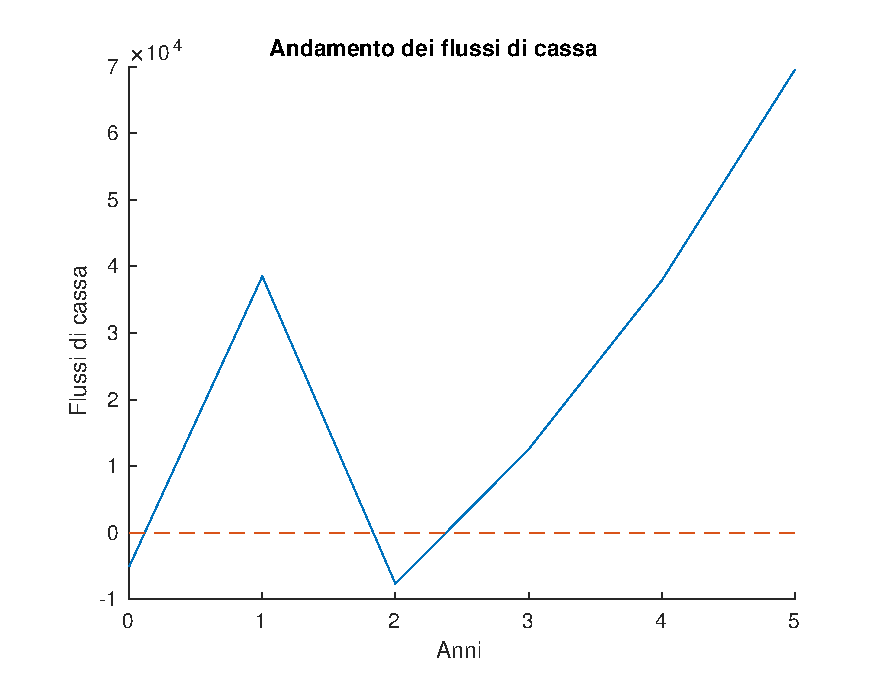
\includegraphics[width=\textwidth]{figures/cf}
\caption{Flussi di cassa scontati relativi primi 5 anni di attività}
\label{cf}
\end{figure}
%
Per ottenere i ricavi netti si calcolano gli OPEX per l’anno di riferimento.
Una loro componente è legata al numero di prodotti realizzati durante l’anno, e
quindi al numero di clienti. Dalla stima precedente risulta un costo unitario di
145.3 \euro/prodotto e comprende i costi relativi ai componenti hardware, alla
spedizione, al box ed ai coloranti. Tale valore è stato moltiplicato per il
numero di nuovi clienti dell’anno di riferimento, ottenendo la spesa totale
legata alla domanda.
A questo costo parziale sono aggiunte le altre componenti annuali degli OPEX,
cioè utenze, stipendi e affitto dell’immobile. Dividendolo per il numero di
nuovi clienti attesi durante l’anno si trova il valore degli OPEX in
\euro/utente. In sintesi:
\begin{displaymath}
	OPEX_{utente} = \frac{\mu \ q(i) + OPEX_{fisso}}{q(i)} = \mu +
    \frac{OPEX_{fisso}}{q(i)}
\end{displaymath}
Ad ogni anno i ricavi netti sono il risultato del prodotto tra ricavo netto per
utente e numero medio di nuovi utenti, secondo la relazione:
\begin{displaymath}
	R_i = (ARPU - OPEX_{utente}) \ q(i)
\end{displaymath}
dove l’ARPU corrisponde al ricavo medio derivante da un singolo utente, quindi
al solo prezzo di acquisto del prodotto.  Il ricavo negativo all’anno 2 è dovuto
quindi al significativo crollo di utenti, i quali risultano insufficienti ad
ammortizzare i costi fissi annuali.
%%%%%%%%%%%%%%%%%%%%%%%%%%%%%%%%%%%%%%%%%%%%%%%%%%%%%%%%%%%%%%%%%%%%%%%%%%%%%%%
%%%%%%%%%%%%%%%%%%%%%%%%%%%%%%%%%%%%%%%%%%%%%%%%%%%%%%%%%%%%%%%%%%%%%%%%%%%%%%%%
%%%%%%%%%%%%%%%%%%%%%%%%%%%%%%%%%%%%%%%%%%%%%%%%%%%%%%%%%%%%%%%%%%%%%%%%%%%%%%%%
%%%%%%%%%%%%%%%%%%%%%%%%%%%%%%%%%%%%%%%%%%%%%%%%%%%%%%%%%%%%%%%%%%%%%%%%%%%%%%%%
\subsection{VAN e TIR}
Abbiamo ipotizzato di effettuare un investimento iniziale $C_0 = 80.000$ e ne 
teniamo conto nel VAN calcolato a $t=0$.
I flussi di cassa, derivanti dalla differenza tra guadagno netto e costi
ricorrenti, dall’anno $t=0$ a $t=5$ sono rappresentati nella
tabella~\ref{tab:van} insieme al VAN cumulativo.\\
Il VAN è calcolato come
\begin{displaymath}
VAN = - C_0 + \sum_{i=1}^n \frac{F_i}{(1 + r)^i}
\end{displaymath}
\begin{eqnarray*}
C_0 &:=& \mbox{investimento iniziale} \\
r &:=& \mbox{tasso di sconto} \\
n &:=& \mbox{numero di periodi analizzati} \\
F_i &:=& \mbox{flusso di cassa relativo al periodo i}
\end{eqnarray*}
% tabella van
\begin{table}[!h]
\centering
%\begin{adjustbox}{width=\textwidth}
\begin{tabular}{c|r@{.}l|r@{.}l}
Anno
& \multicolumn{2}{|c}{$F_i$ [\euro]}
& \multicolumn{2}{|c}{VAN [\euro]}
\\          
\hline
0 & -5080&00 & -85080&00 \\
1 & 38512&84 & -46567&16 \\ 
2 & -7652&85 & -54220&01 \\
3 & 12528&92 & -41691&09 \\
4 & 37858&96 &  -3832&13 \\
5 & 69519&19 &  \textbf{65687}&\textbf{06} 
\end{tabular}
%\end{adjustbox}
\caption{Valore Attuale Netto}
\label{tab:van}
\end{table}

%
\begin{figure}[!h]
\centering
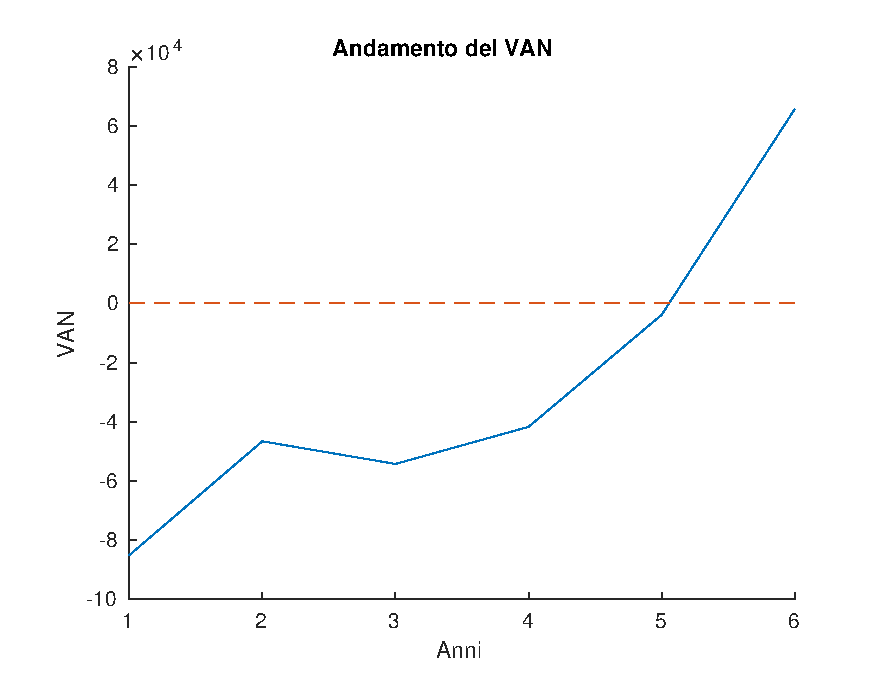
\includegraphics[width=\textwidth]{figures/van}
\caption{Andamento del VAN nei primi 5 anni di attività}
\label{van}
\end{figure}
%
Otteniamo VAN = 65687.06 nell'anno $t=5$. All'anno $t=2$ si può osservare una
diminuzione del VAN rispetto all'anno precedente. Questa è imputabile alla
diminuzione del numero di clienti rispetto all'anno $t=1$. Infatti, come detto
in precedenza, il numero di clienti non è una funzione cumulativa.

Il periodo di pareggio finanziario (payback period) è dunque raggiunto tra il
quarto ed il quinto anno. Essendo un indice che può essere interpretato come
grado di rischio associato al progetto, ci si può ritenere soddisfatti di poter
mostrare che entro il quinto anno di esercizio la nostra azienda può raggiungere
il pareggio e ottenere un VAN positivo.

Il TIR è il tasso di attualizzazione per cui il VAN del progetto è pari a zero, 
ed è usato per misurare la redditività e la robustezza di progetti e investimenti.
Studiando il valore del VAN al variare del tasso di sconto, e riducendo
l’intervallo ricercando di volta in volta il valore del VAN nel punto medio,
si è giunti all’intervallo \mbox{$[0.285, 0.286]$}. Il valore del VAN agli estremi è
$VAN(r = 28.5\%) = 407.86 \mbox{\euro}$ e $VAN(r=28.6) = -570.56 \mbox{\euro}$,
dunque scegliendo il punto intermedio abbiamo definito come valore il $TIR = 28.55\%$.

Dai risultati ottenuti possiamo notare che il progetto è potenzialmente positivo
visto l'esito dei flussi di cassa. Il calcolo del VAN prevede che entro il quinto
anno di attività si dovrebbe raggiungere il pareggio finanziario, coprendo
dunque l’investimento iniziale e le spese dei primi anni di attività e
raggiungendo una situazione di attivo tra costi e ricavi.  Inoltre dal confronto
tra WACC e TIR possiamo dedurre se è conveniente investire o meno nel nostro
progetto. Poiché il TIR è sufficientemente grande affinché il progetto resista
a eventuali fluttuazioni del tasso di sconto si può concludere che è
conveniente.
%%%%%%%%%%%%%%%%%%%%%%%%%%%%%%%%%%%%%%%%%%%%%%%%%%%%%%%%%%%%%%%%%%%%%%%%%%%%%%%%
%%%%%%%%%%%%%%%%%%%%%%%%%%%%%%%%%%%%%%%%%%%%%%%%%%%%%%%%%%%%%%%%%%%%%%%%%%%%%%%%
%%%%%%%%%%%%%%%%%%%%%%%%%%%%%%%%%%%%%%%%%%%%%%%%%%%%%%%%%%%%%%%%%%%%%%%%%%%%%%%%
%%%%%%%%%%%%%%%%%%%%%%%%%%%%%%%%%%%%%%%%%%%%%%%%%%%%%%%%%%%%%%%%%%%%%%%%%%%%%%%%
\subsection{Valutazione del rischio}
I rischi individuati per il prodotto in relazione alla loro natura sono:
\begin{itemize}
\item Rischi puri: incendi, terremoti, guasti nelle attrezzature;
\item Rischi speculativi: oscillazione dei tassi di cambio, innovazioni
tecnologiche (per esempio rappresentate dall’utilizzo di droni), variazioni nel
costo dell’hardware, variazione di costi operativi.
\end{itemize}

Sono stati valutati una serie di rischi significativi, analizzando singolarmente
l’incidenza sull’andamento del VAN. Non si è tenuto conto del rischio di
incendi in quanto molto basso in percentuale nel nostro caso, visto che la
probabilità di incendio viene calcolata in base diretta al numero di dipendenti,
la grandezza dell’immobile e la quantità di materiale infiammabile. Il rischio
per terremoti non è stato considerato in quanto, ipotizzando di avere la nostra
società a Roma, siamo in un’area con bassa probabilità di attività sismica.

Per osservare l’incidenza di ogni fattore di rischio si fissata una
percentuale di variazione dei parametri associati pari al 10\%. Si è quindi
calcolato il VAN sia nel caso in cui tale variazione sia positiva che negativa,
e si è determinata la sua variazione percentuale rispetto al VAN ottenuto nel
caso “reale”.

I risultati sono rappresentati nel “diagramma tornado” in figura~\ref{tornado} e
nella tabella~\ref{tab:risk}, che mostrano i fattori di rischio ordinati in base
alla loro incidenza sul VAN.
\begin{table}[!h]
\centering
%\begin{adjustbox}{width=\textwidth}
\begin{tabular}{c|c|c|r@{.}l|r@{.}l}
& Valore 
&
& \multicolumn{2}{|c}{}
& \multicolumn{2}{|c}{Percentuale}
\\
Parametro
& attuale
& Variazione 
& \multicolumn{2}{|c}{VAN [\euro]}
& \multicolumn{2}{|c}{variazione}
\\

\hline
Domanda    &            &                          & 50780&78 & 271&67\%  \\
           &            &                          &-23456&60 &-271&68\%  \\
\hline                                  
Costo      & \EUR{1000} & $ + 100 \ \mbox{\euro} $ &  8441&81 & -38&21\%  \\
affitto    &            & $ - 100 \ \mbox{\euro} $ & 18885&13 & +38&22\%  \\
\hline                  
Costo      & \EUR{115}  & $+ 11.5 \ \mbox{\euro} $ & 38342&71 & 180&63\%  \\
hardware   &            & $- 11.5 \ \mbox{\euro} $ &-11016&67 &-180&63\%  \\
\end{tabular}
%\end{adjustbox}
\caption{Variazione del VAN al variare dei parametri coinvolti dai rischi}
\label{tab:risk}
\end{table}

%
\begin{figure}[!h]
\centering
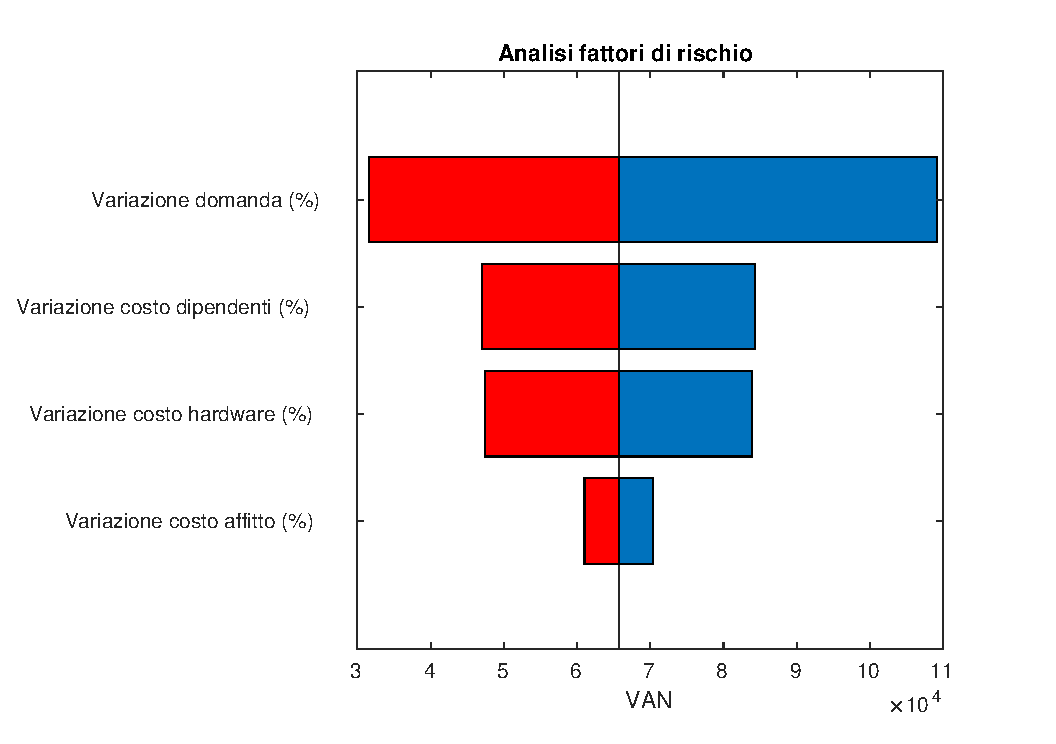
\includegraphics[width=\textwidth]{figures/tornado}
\caption{Diagramma tornado associato ai rischi}
\label{tornado}
\end{figure}
%
Il fattore di rischio con incidenza maggiore è dunque rappresentato dalla
“variazione della domanda”. La “variazione del costo per gli stipendi” e il
“costo dell’hardware” hanno un’incidenza media, mentre il “costo relativo
all’affitto” ha un’incidenza minore.
%%%%%%%%%%%%%%%%%%%%%%%%%%%%%%%%%%%%%%%%%%%%%%%%%%%%%%%%%%%%%%%%%%%%%%%%%%%%%%%%
%%%%%%%%%%%%%%%%%%%%%%%%%%%%%%%%%%%%%%%%%%%%%%%%%%%%%%%%%%%%%%%%%%%%%%%%%%%%%%%%
%%%%%%%%%%%%%%%%%%%%%%%%%%%%%%%%%%%%%%%%%%%%%%%%%%%%%%%%%%%%%%%%%%%%%%%%%%%%%%%%
%%%%%%%%%%%%%%%%%%%%%%%%%%%%%%%%%%%%%%%%%%%%%%%%%%%%%%%%%%%%%%%%%%%%%%%%%%%%%%%%
